\documentclass[pdftex,10.5pt]{report}
\usepackage{amsmath}
\usepackage{caption}
\usepackage{graphicx}
\usepackage{import}
\usepackage[hmargin=.97in,vmargin=.97in]{geometry}
\usepackage{hyperref}
\usepackage{cleveref}
\usepackage{multicol}
\usepackage[square,sort,comma,numbers]{natbib}
\usepackage[abs]{overpic}
\usepackage{setspace}
\usepackage{subcaption}
\usepackage{wrapfig}
\usepackage{listings}


\renewcommand*\thesection{\arabic{section}}

\makeatletter
\renewcommand\bibsection{
  \section*{\refname
    \@mkboth{\MakeUppercase{\refname}}{\MakeUppercase{\refname}}}
}
\makeatother

\onehalfspacing

\begin{document}

%%%%%%%%%%%%%%%%%%%%%%%%%%%%%%%%%%%%%%%%%
% University Assignment Title Page 
% LaTeX Template
%
% This template has been downloaded from:
% http://www.latextemplates.com
%
% Original author:
% WikiBooks (http://en.wikibooks.org/wiki/LaTeX/Title_Creation)
%%%%%%%%%%%%%%%%%%%%%%%%%%%%%%%%%%%%%%%%%
\begin{titlepage}

\newcommand{\HRule}{\rule{\linewidth}{0.5mm}} % Defines a new command for the horizontal lines, change thickness here

\center % Center everything on the page
 
%----------------------------------------------------------------------------------------
%	HEADING SECTIONS
%----------------------------------------------------------------------------------------

\textsc{\LARGE Rutgers, the State University of New Jersey}\\[1.5cm] % Name of your university/college
\textsc{\Large Independent Study / Special Problems}\\[0.5cm] % Major heading such as course name
%\textsc{\large Minor Heading}\\[0.5cm] % Minor heading such as course title

%----------------------------------------------------------------------------------------
%	TITLE SECTION
%----------------------------------------------------------------------------------------

\HRule \\[0.4cm]
{ \huge \bfseries FPGA Design}\\[0.4cm] % Title of your document
\HRule \\[1.5cm]
 
%----------------------------------------------------------------------------------------
%	AUTHOR SECTION
%----------------------------------------------------------------------------------------

\begin{minipage}{0.4\textwidth}
\begin{flushleft} \large
\emph{Author:}\\
Elie \textsc{Rosen} % Your name
\end{flushleft}
\end{minipage}
~
\begin{minipage}{0.4\textwidth}
\begin{flushright} \large
\emph{Advisor:} \\
Professor Michael \textsc{Caggiano} % Supervisor's Name
\end{flushright}
\end{minipage}\\[4cm]


%----------------------------------------------------------------------------------------
%	DATE SECTION
%----------------------------------------------------------------------------------------

{\large \today}\\[3cm] % Date, change the \today to a set date if you want to be precise

%----------------------------------------------------------------------------------------
%	LOGO SECTION
%----------------------------------------------------------------------------------------

%\includegraphics{Logo}\\[1cm] % Include a department/university logo - this will require the graphicx package
 
%----------------------------------------------------------------------------------------

\vfill % Fill the rest of the page with whitespace

\end{titlepage}

\begin{abstract}
The Intel 8086 microprocessor was first introduced in 1978. Since then the semiconductor industry has changed vastly from the old chip manufacturing techniques of the time. Today we can fit thousands of Intel 8086 microprocessors in the same size package with use of modern semiconductor techniques such as the ability to design with 22nm feature size and better yield from improved wafer quality. This paper examines how we can still learn from preceding technology with a more modern twist. By utilizing field programmable gate arrays, we can easily implement the same technology from the past and learn about architectures that are still relevant in todays modern processors.
\end{abstract}

\tableofcontents

\section{Introduction}
It was in the mid 1970s when Intel announced their latest project, the Intel 8086 -  a 16-bit microprocessor capable of supporting up to a revolutionary 1 mega{\em byte} of address space and 64 kilo{\em bytes} of input/output. Gone were the days of simple computing in only 8-bits of freedom, this was the 70's and 16-bits were here to take over. Along with the increases in accessible memory and larger size ALU computations, Intel introduced a new type of architecture and instruction set known as x86, this new method of computing revolved around the use of registers that stored input and output data which could then have computations performed on them. This improvement has since paved the way for future computing by setting a standard on how the processor receives data and how the data can then be processed in a regular clock cycle. The 8086 supported 80 assembly instructions which also included instructions compatible with the older 8-bit processors so the older programs would still be backwards compatible with the new technology, this capability alone was one of the major reasons that large companies began transitioning to the new architecture which began a substantial drive to future 16-bit iterations of the processor.

The field-programmable gate array (FPGA) has been around since the 1980's, its purpose was to be able to easily create and prototype custom hardware without having to expend vast resources required for designing and manufacturing application-specific integrated circuits (ASICs). The FPGA accomplishes this by using "logic elements" (LE), a term that varies by manufacturer but is essentially the same, which is typically a circuit that consists of a lookup table for performing an array of logic operations,  multiplexers and low level logic gates that can be configured in such a way as to create custom complex logic such as adders/subtractors or even be used for more simple XOR and NAND gates. A common structure of a logic element can be found in Figure \ref{fig:LogicElement}, this one is from the Altera Cyclone III family. The elements  are most often configured as a matrix with interconnects for inputs, outputs and configuration paths in between. In the last decade or so, improvements in silicon technologies have allowed FPGA manufacturers to greatly increase the number of logic elements on a chip into the hundreds of thousands and beyond which makes it possible to design hardware of almost the same complexity as modern ASICs.

\begin{figure}[!h]
	\centering
	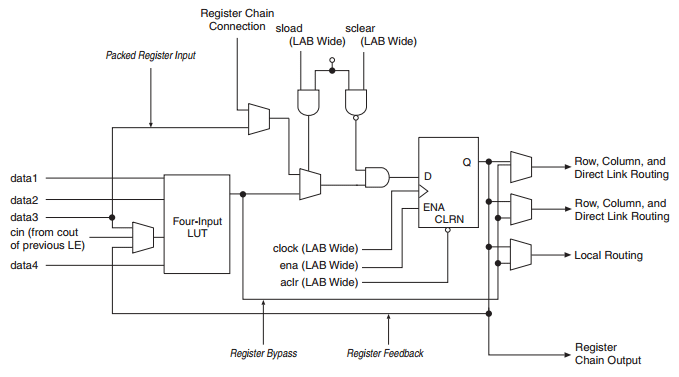
\includegraphics[width=3.5in]{figures/LogicElement.png}
	\caption{Cyclone III Device Family LEs in Normal Mode \cite{CycloneHandbook}}
	\label{fig:LogicElement}
\end{figure}

After discovering an independent open source initiative, Zet Processor - a clone of the Intel 8086 hardware description by Zeus Gómez Marmolejo, it was determined that this project would make it possible so that the Intel 8086 microprocessor could be implemented onto a modern FPGA \cite{ZetProcessor}. The project as a whole would encourage study in all areas of focus for a person with primary interests in Computer Architecture, Digital Systems Design, FPGAs, and Assembly programming. This project and study  is something that can also be completed within the time frame of a typical academic semester.

\section{Implementation Requirements}
Through extensive research of various FPGA manufacturers and the different styles of development boards offered from a select number of companies, it was determined that an FPGA that is able to hold more than 9,000 LEs would be required to successfully implement the Intel 8086 microprocessor. As an added necessity, it was important to select a development board that would be able to handle the project inputs and outputs such as PS2 keyboard and VGA output in order to spend more time on the study and not building miscellaneous external hardware. From this research, it was determined that the Altera DE0 development board sufficiently met the project needs with over 15,000 LE's, a VGA port, a PS2 port, buttons, LEDs, switches, and USB interface. Another important addition to the board is its Secure Digital (SD) memory card slot which would allow for external flash memory storage of an operating system, full specifications for the Altera DE0 board can be found in Appendix \ref{App:AppendixA}.

Other components for the project include; an LCD monitor to visualize the system status, a PS2 keyboard to interact with the operating system, a computer with Linux to compile the processor and write the operating system to the memory card.

Since the study is sponsored by the Altera University Program, an Altera DE0 development board has been provided as well as an Altera DE0-Nano development boards at no cost. This makes the projects overall required budget \$0 since the devices come with the necessary software to program the FPGA and all of the other software packages used are open source.

\section{Procedure}
The Zet Processor is more than just Verilog code for an Intel 8086 microprocessor, it also contains the necessary BIOS and drivers for treating the SD memory card as a mounted hard disc. The preliminary steps for installing the processor first include compiling the BIOS by running it through the Open Watcom compiler which takes the BIOS code written in C and compiles it into x86 Assembly optimized for 16-bit instructions \cite{Watcom}. We then take the BIOS assembly and convert it into hexadecimal by means of a simple file conversion script, this is now our ROM for placing onto the FPGA. The BIOS then gets placed onto the FPGA through running the DE0\_Control\_Panel, an example program that comes with the FPGA software, which allows for files to be placed directly onto the on-board flash memory. This is important because as the processor boots, it will automatically look at address 0x00000 for instructions on where to next proceed such as how to mount the operating system and ultimately boot it. 

Since the processor runs 16-bit x86 it is necessary to choose a compatible operating system. This leaves a few options including MS-DOS 6.22, FreeDOS 1.1, and Microsoft Windows 3.0. MS-DOS was chosen due to its small file size and easy to work with command line interface, as an added bonus the copyright for MS-DOS has expired which makes it very easy and convenient to find the source code in various places on the Internet. To load the operating system, it was necessary to load the files exactly as described from the downloaded image. The process was accomplished by running {\tt dd if=./msdos.img of=/dev/sdc} on a Linux computer, this instruction mounts the MS-DOS image byte-by-byte onto the SD memory card which is necessary for when the BIOS looks at a specific memory location to start the operating system.

In order to begin the process of loading the Zet Processor hardware onto the FPGA, it is first important to read the documentation and manuals for the Altera DE0 Development Board and accompanying Quartus II software manual. 

The process for loading Verilog onto the device is fairly straightforward, that is to compile the Verilog code and debug any miscellaneous warnings and compilation errors and then to utilize the on-board programmer to load the code onto the device. When loading the code it is important to take note of the different ways in which the code can be loaded. If the code is loaded through the Joint Tag Action Group (JTAG) interface, it is important to note that this only temporarily loads the hardware and all progress will be lost after powering down the device. This feature is due to the fact that JTAG is made for testing and only loads values directly into the flip-flops and accompanying hardware but does not save this setup data to the flash memory. Since this method only sets the hardware, it can load the hardware almost instantaneously. The other method for loading hardware is known as Active Serial programming (AS), this method requires that the FPGA device is placed into programming mode which can be done by flipping a switch placed on the development board. AS places the FPGA configuration data into FLASH memory which is read into the device at power up.

\begin{figure}[!h]
	\centering
	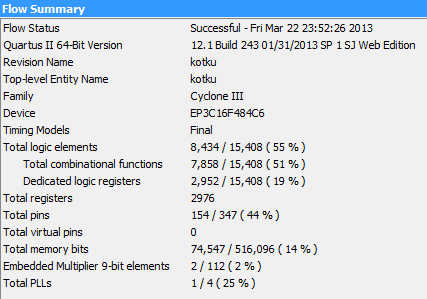
\includegraphics[width=3.5in]{figures/CompileResults.png}
	\caption{Compilation results of the Zet Processor from Quartus II software.}
	\label{fig:CompileResults}
\end{figure}

\section{Results}
After performing the necessary steps as described by the procedure, the processor is now fully functional and can run an operating system as shown in Figure \ref{fig:WorkingFPGA}. This was the primary objective for the project and is considered to define the project as an overall success. The next steps were to design presentation materials for demonstration, since MS-DOS includes a program called QBASIC which is a BASIC language interpreter based off of Microsoft's more popular software QuickBASIC, some demonstration programs were written to show off some of the processors capabilities such as the Hello World program and a small game for guessing a random number. The operating system also included some games which could be played through keyboard input such as Rogue, which is described as a crawling dungeon game with ASCII text based graphics that are easily displayed in terminal where the player has to fight off goblins only disguised as the letter "G" and collect coins throughout the map \cite{Rogue}. 

\begin{figure}[!h]
	\centering
	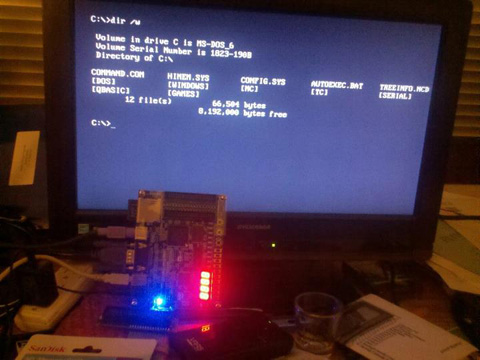
\includegraphics[width=3in]{figures/fpgaworking.jpg}
	\caption{FPGA loaded with an Intel 8086 microprocessor running MS-DOS 6.22}
	\label{fig:WorkingFPGA}
\end{figure}

\section{Problems Faced \& Troubleshooting}
The number one challenge in completing this study was a lack of full documentation and user base for the Zet Processor. It became evident very early on in research that this project would require extensive digging through the source code and custom modifications to get it to work with the Cyclone III device. The last update for the project was over a year ago and the online support forums provided little resource with many of the problems faced when trying to implement the processor. It was also difficult to determine which version of the processor was relevant to the documentation so it was assumed that most of what was found was obsolete or not correct.

Issues in implementing the processor involved problems with the BIOS not compiling due to Open Watcom not being correctly added to the system path, once this was resolved the BIOS compiled correctly. The installation document also does not make clear that it is necessary to convert the BIOS into hexadecimal, when this was done and added into the ROM the processor behaved correctly. 

There were also some stability issues with the SD memory, the project site lists a way to mount MS-DOS to the SD card through a program known as Winimage but this failed multiple times and always left the processor hung up at different parts of the boot sequence. This was corrected by loading instead the image byte-by-byte in Linux as mentioned previously, which was not as simple as it sounds since there were also issues with the SD card not being formatted properly. It was finally fixed by formatting the card with all zeros and then the operating system began to work properly.

Lastly, once MS-DOS was finally operational after quite a few hours of debugging it was powered down for the evening and then turned back on in the morning, the result was an error stating that the SD card had become corrupt. This was odd due to the fact that it was operational not but a few hours beforehand. After power cycling the device a few times and with feelings of great defeat that the processor was still not functional, a last ditch effort of removing the SD card and blowing air into the slot and placing the card back into the slot was attempted. The device was then powered back on and worked flawlessly.

\section{Conclusion}
One of the primary objectives for this study was to gain comprehensive knowledge of the inner working of FPGAs and x86 architecture. By working with the Zet Processor as a working clone of the Intel 8086 hardware it was possible to complete this research within the course of one academic semester. Through this research, it has become clear that a project of this complexity can adequately prepare a person to learn the inner workings of FPGAs. The process of compiling and debugging an early processor gives experience in how to manage a design where hardware may sometimes be limited. It also examines topics in low level device drivers and memory management. Working with the original x86 architecture from the 1970's provided great insight into its relation to the 32-bit and 64-bit versions of x86. It is very clear to see how the industry has changed so much during this time but yet, many of the artifacts from 16-bit architecture are still present in modern versions. Overall, the fact that technology from long ago can still be examined through more modern means such as through FPGAs allows for the technology to continue to be explored and aids in giving great experience in computer architecture design to students interested in pursuing this area of study.

% use section* for acknowledgment
\section*{Acknowledgment}
The author would like to thank the Altera University Program \cite{UniProgram} for providing development boards and necessary software for work on this area of study.

\section{Appendix}

\label{App:AppendixA}
\subsection{Full specifications for Altera DE0 development board:}
\begin{itemize}
\item FPGA
	\begin{itemize}
 	\item Cyclone III 3C16 FPGA
	\item 15,408 LEs
	\item 56 M9K Embedded Memory Blocks
	\item 504K total RAM bits
	\item 56 embedded multipliers
	\item 4 PLLs
	\item 346 user I/O pins
	\item FineLine BGA 484-pin package
	\end{itemize}
\item Memory
	\begin{itemize}
	\item SDRAM
		\begin{itemize}
		\item One 8-Mbyte Single Data Rate Synchronous Dynamic RAM memory chip
		\end{itemize}
	\item Flash memory
		\begin{itemize}
		\item 4-Mbyte NOR Flash memory
		\item Support Byte (8-bits)/Word (16-bits) mode
		\end{itemize}
	\item SD card socket
		\begin{itemize}
		\item Provides both SPI and SD 1-bit mode SD Card access
		\end{itemize}
	\end{itemize}
\item Interface
	\begin{itemize}
	\item Built-in USB Blaster circuit
		\begin{itemize}
	 	\item On-board USB Blaster for programming
		\item Using the Altera EPM240 CPLD
		\end{itemize}
	\item Altera Serial Configuration device
		\begin{itemize}
		\item Altera EPCS4 serial EEPROM chip
		\end{itemize}
	\item Pushbutton switches
		\begin{itemize}
		\item 3 pushbutton switches
		\end{itemize}
	\item Slide switches
		\begin{itemize}
		\item 10 Slide switches
		\end{itemize}
	\item General User Interfaces
		\begin{itemize}
		\item 10 Green color LEDs
		\item 4 seven-segment displays
		\end{itemize}
	\item Clock inputs
		\begin{itemize}
		\item 50-MHz oscillator
		\end{itemize}
	\item VGA output
		\begin{itemize}
		\item Uses a 4-bit resistor-network DAC
		\item With 15-pin high-density D-sub connector
		\item Supports up to 1280x1024 at 60-Hz refresh rate
		\end{itemize}
	\item Serial ports
		\begin{itemize}
		\item One RS-232 port (Without DB-9 serial connector)
		\item One PS/2 port
		\end{itemize}
	\item Two 40-pin expansion headers
		\begin{itemize}
		\item 72 Cyclone III I/O pins, as well as 8 power and ground lines, are brought out to two 40-pin expansion connectors
		\item40-pin header is designed to accept a standard 40-pin ribbon cable used for IDE hard drives
		\end{itemize}
	\end{itemize}
\end{itemize}

\label{App:AppendixB}
\subsection{Available x86 Instructions on the Zet Processor:}

{\noindent\bf Data transfer instructions} \\
mov, push/pop, in/out, lahf/sahf, lds/lea/les, pushf/popf, xchg, xlat

{\noindent\bf Arithmetic instructions} \\
aaa/aas, aam, aad, daa/das, cbw/cwd, inc, dec, add/adc, sub/sbb, mul/imul, div/idiv, neg, cmp

{\noindent\bf Bitwise handling instructions} \\
and/or, not, rcl, rcr, rol, ror, sal/shl, sar, shr, test, xor

{\noindent\bf Control transfer instructions} \\
call, ja/jnbe, jae/jnb/jnc, jb/jnae/jc, jbe/jna, jcxz, je/jz, jg/jnle, jge/jnl, jl/jnge, jle/jng, jne/jnz, jno, jnp/jpo, jns, jmp, jo, jp/jpe, js, loop, loope/loopz, loopne/loopnz, ret

{\noindent\bf String handling instructions}\\
cmpsb/cmpsw, lodsb/lodswm, movsb/movsw, rep (pref), repe/repz (pref), repne/repnz (pref), scasb/scasw, stosb/stosw

{\noindent\bf Interrupt instructions} \\
int, into, iret

{\noindent\bf Microprocessor control instructions} \\
clc, cld, cli, cmc, hlt, nop, stc, std

\subsection{Processor BIOS}
\lstset{numbers=left, stepnumber=2, frame=single, breaklines=true}
\lstinputlisting[language={[ANSI]C}]{code/zetbios.c} 

\subsection{Hardware Description for FPGA RAM}
\lstinputlisting[language=Verilog]{code/WB_Flash.v} 

\subsection{Hardware Description for Loading Static ROM}
\lstinputlisting[language=Verilog]{code/BIOSROM.v} 

% references section
{\footnotesize\singlespacing
\bibliographystyle{IEEEtran}
\bibliography{FinalReport}
}

\end{document}